This exercise has been completed in the attached \textit{K\_Means.ipynb} Jupyter Notebook. The most relevant bits of source code can be seen here as well, though all comments are left out. It should be noted that the code for this is the exact same as in the previous subexercise, except the "model.fit(image)" line has been exchanged for the following. The full source code is in the notebook:
\begin{verbatim}
if (imgx*imgy > 50000):
        modLen = 5000

        temp = np.arange(0,(imgx*imgy),1).reshape((imgx*imgy))
        smallImgInd = np.random.choice(temp, modLen, False)
        
        smallImg = image[smallImgInd]

        model.fit(smallImg)
        model.cluster_assignments = 
            model.assign_to_clusters(image, model.cluster_means)
    else:
        model.fit(image)
\end{verbatim}
The 16 cluster means, calculated using the Jupyter Notebook, look as follows. It should be noted that the cluster means have been calculated by choosing 5000 random pixels in the image, and fitting the model to those instead of the entire image. Doing it this way should only have a minimal effect on the result, if 5000 pixels are enough to find a representative of the image. It should also be noted that they are all RGB values, but Python wants RGB values in one of two forms; floats between $0$ and $1$, or integers between $0$ and $255$. Here they are floats between $0$ and $1$:\\
$$
\begin{matrix}
[0.49441064, 0.46930358, 0.42724814] \\[3pt]
[0.31073644, 0.29808085, 0.27156238] \\[3pt]
[0.66100118, 0.82807700, 0.88582735] \\[3pt]
[0.44086687, 0.80361197, 0.43168215] \\[3pt]
[0.76419118, 0.74735294, 0.69117647] \\[3pt]
[0.07393128, 0.06195302, 0.06012036] \\[3pt]
[0.65701033, 0.44427577, 0.18943707] \\[3pt]
[0.58076367, 0.58930857, 0.57473684] \\[3pt]
[0.94262126, 0.81946042, 0.34577621] \\[3pt]
[0.25930767, 0.37516340, 0.48351489] \\[3pt]
[0.19096334, 0.59283887, 0.85473146] \\[3pt]
[0.59541250, 0.66392897, 0.70810211] \\[3pt]
[0.42336683, 0.77392124, 0.89866355] \\[3pt]
[0.45891803, 0.51344200, 0.56130404] \\[3pt]
[0.71649763, 0.62609872, 0.47396890] \\[3pt]
[0.92123446, 0.95420905, 0.95794388]
\end{matrix}
$$
The assigned cluster for each pixel has been calculated, and the new image has been plotted:\\
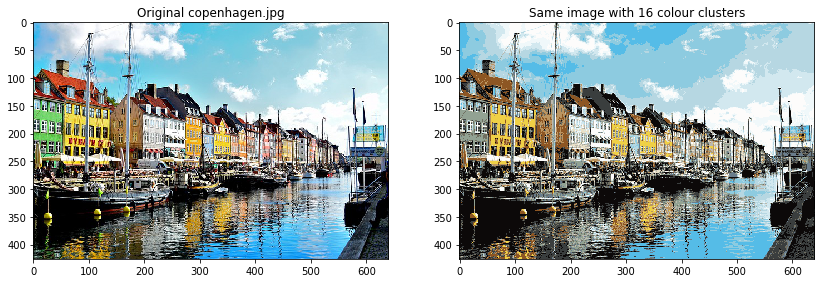
\includegraphics[width=\linewidth]{3c1.png}\\